\documentclass[conference]{IEEEtran}
\IEEEoverridecommandlockouts
% The preceding line is only needed to identify funding in the first footnote. If that is unneeded, please comment it out.
\usepackage{cite}
\usepackage{amsmath,amssymb,amsfonts}
\usepackage{algorithmic}
\usepackage{graphicx}
\usepackage{textcomp}
\usepackage{xcolor}
\usepackage{svg}
\def\BibTeX{{\rm B\kern-.05em{\sc i\kern-.025em b}\kern-.08em
    T\kern-.1667em\lower.7ex\hbox{E}\kern-.125emX}}
\begin{document}

\title{Hybrid Long-Term Object Tracking (HLT-MOT) System\\
% {\footnotesize \textsuperscript{*}Note: Sub-titles are not captured in Xplore and
% should not be used}
% \thanks{Identify applicable funding agency here. If none, delete this.}
}

\author{\IEEEauthorblockN{Nafis Ahmed}
\IEEEauthorblockA{\textit{Department of Information Technology} \\
\textit{FH Dortmund}\\
Dortmund, Germany \\
nafis.ahmed@fh-dortmund.de}
\and
\IEEEauthorblockN{Björn Schäfer}
\IEEEauthorblockA{\textit{Department of Information Technology} \\
\textit{FH Dortmund}\\
Dortmund, Germany \\
bjoern.schaefer@fh-dortmund.de}
\and
\IEEEauthorblockN{Hugues Tchouankem}
\IEEEauthorblockA{\textit{Department of Information Technology} \\
\textit{FH Dortmund}\\
Dortmund, Germany \\
hugues.tchouankem@fh
dortmund.de}
}

\maketitle

\begin{abstract}
This paper presents a Hybrid Long-Term Object Tracking (HLT-MOT) system that effectively addresses the challenges of maintaining object identities over extended periods, particularly during occlusions or temporary disappearances. Our approach combines DeepSORT's frame-to-frame tracking capabilities with a robust re-identification framework powered by DINOv2 deep learning model. The system maintains feature galleries for tracked objects and employs both online and offline re-identification strategies to recover lost identities. Key innovations include: (1) a dual-model approach that balances accuracy and computational efficiency, (2) GPU-accelerated batch processing for feature extraction and matching, (3) Numba-optimized spatial-temporal consistency checks, and (4) dedicated mechanisms for prioritized tracking of a primary object. Experimental results demonstrate that our system significantly outperforms traditional tracking approaches in challenging scenarios involving long-term occlusions, crowded scenes, and appearance changes, while maintaining near real-time performance. The HLT-MOT system has important applications in surveillance, autonomous navigation, and human-computer interaction domains where persistent identity tracking is essential.
\end{abstract}

\begin{IEEEkeywords}
Multi-Object Tracking, Long-Term Tracking, Re-identification, DeepSORT, Feature Extraction, Object Detection, Computer Vision
\end{IEEEkeywords}

\section{Introduction}
Robust, long-term person tracking is a cornerstone of intelligent systems in a multitude of applications, from human-robot collaboration and autonomous navigation to security and surveillance. The fundamental challenge lies not merely in following a person in an uncluttered view, but in maintaining a consistent identity through complex, real-world scenarios. These scenarios are characterized by frequent and prolonged occlusions, significant variations in appearance due to changing viewpoints and lighting, and the presence of visually similar distractors. Traditional tracking systems, which often couple a detector like YOLO \cite{7780460} with a motion-centric tracker such as DeepSORT \cite{Wojke2017simple,Wojke2018deep}, perform well in short-term scenarios but often fail when an object reappears after a long absence, as their underlying feature representations lack the robustness to bridge significant appearance gaps \cite{10623162}. The recent advent of large-scale, self-supervised foundation models has marked a paradigm shift in visual perception, enabling unprecedented performance on open-set recognition tasks. Works such as "Follow Anything" \cite{maalouf2023follow} have demonstrated the power of models like DINO \cite{DBLP:journals/corr/abs-2104-14294} and SAM \cite{10378323} to track arbitrary objects specified by a user query in real-time. Inspired by this progress, our work specializes these powerful representations for the specific and demanding task of long-term person re-identification (Re-ID). In this paper, we present a hybrid, real-time person tracking and re-identification system designed for long-term identity persistence. Our system synergistically combines the motion-prediction efficiency of DeepSORT for short-term tracking with a powerful appearance-based re-identification module built upon the DINOv2 \cite{oquab2023dinov2,darcet2023vitneedreg,jose2024dinov2meetstextunified} vision transformer. The core of our approach lies in a mask-aware feature extraction pipeline. By leveraging a segmentation-capable detector (YOLOv8-Seg) \cite{Jocher_Ultralytics_YOLO_2023,10533619}, our system extracts discriminative features exclusively from the pixels of the segmented person, rather than the entire bounding box. This technique significantly improves feature quality and robustness against background clutter, a common failure point for traditional Re-ID methods. To ensure real-time applicability, the entire system is heavily optimized, employing TensorRT-accelerated \cite{nvidia_tensorrt} detection, batched GPU computations for feature extraction, and Numba-accelerated CPU operations.\\
\textit{Our main contributions are:}
A hybrid tracking architecture that integrates the motion-based tracking of DeepSORT with a robust DINOv2-based appearance gallery for long-term re-identification.
A mask-aware feature extraction pipeline that utilizes segmentation masks to generate superior, clutter-free appearance descriptors for person Re-ID.
An end-to-end, real-time optimized system that demonstrates effective long-term tracking of a primary individual through significant occlusions and appearance changes.

\section{Related Work}
The challenge of robust, long-term multi-object tracking (MOT) has been approached from several angles, evolving from purely motion-based methods to sophisticated deep learning architectures. Our work builds upon established principles while integrating recent advances in self-supervised learning to address the specific demands of long-term person re-identification (Re-ID).
\subsection{Tracking-by-Detection and DeepSORT}
The dominant paradigm in modern MOT is tracking-by-detection, where objects are first detected in each frame and then associated across frames to form trajectories. Early methods like SORT (Simple Online and Realtime Tracking) \cite{Bewley2016_sort} relied solely on motion prediction using a Kalman filter and association based on spatial overlap (IoU), making them fast but susceptible to failures during occlusions or with crowded scenes.
A significant advancement came with DeepSORT \cite{Wojke2017simple,Wojke2018deep} and succssors like StrongSort\cite{Bewley2016_sort}, which extended SORT by incorporating an appearance-based metric. DeepSORT trains a separate deep neural network to extract appearance features from each detected object. The association cost matrix is then computed as a weighted sum of motion similarity (Mahalanobis distance) and appearance similarity (cosine distance of feature embeddings). This hybrid approach makes the tracker more robust to short-term occlusions where motion prediction might be unreliable. As demonstrated in various robotic systems, including the person-following robot by Zhang et al.\cite{10623162}, the combination of a detector like YOLO and a tracker like DeepSORT forms a potent baseline for tracking tasks. Our HLT-MOT system adopts DeepSORT's efficient motion prediction and frame-to-frame association mechanism as its foundation for short-term tracking.
\subsection{Long-Term Re-identification and its Challenges}
While DeepSORT's appearance model improves short-term tracking, its lightweight Re-ID network often lacks the robustness required to re-associate an object after a prolonged absence, significant viewpoint changes, or severe illumination variations. This is a common failure point in real-world scenarios, leading to identity switches and fragmented tracks. As noted by Zhang et al\cite{10623162}. in the context of robot person following, a fixed feature extractor often fails to generalize across the diverse appearances encountered during a long interaction, a problem known as domain drift.
This limitation has spurred research into more powerful Re-ID techniques. However, many state-of-the-art Re-ID models are designed for multi-camera surveillance datasets and are computationally too expensive to integrate directly into a real-time, single-camera tracking loop. Our work directly confronts this challenge by designing a system that can bridge these long-term appearance gaps without sacrificing real-time performance.
\subsection{Foundation Models for Visual Representation}
The recent advent of large-scale, self-supervised foundation models has revolutionized visual perception. Models like DINO (self-distillation with no labels) [6] and its successor, DINOv2 [8], have demonstrated an extraordinary ability to learn highly discriminative and semantically rich visual features without human-annotated labels. These features exhibit remarkable robustness to viewpoint, scale, and appearance changes, making them ideal for challenging Re-ID tasks.
Recent works like "Follow Anything" (FAn) by Maalouf et al. [5] have shown the potential of these models for open-set tracking. The FAn system leverages foundation models like DINO and SAM (Segment Anything Model) [7] to detect, track, and follow arbitrary, user-specified objects in real-time. This highlights a paradigm shift from using task-specific models to leveraging general-purpose, powerful visual representations. Inspired by this progress, our HLT-MOT system specializes this approach for the demanding and specific task of long-term person Re-ID. Instead of open-set tracking, we harness the power of DINOv2 to create a highly robust "visual fingerprint" specifically for identifying individuals, enabling our system to maintain identity even after long and complex occlusions.
\subsection{Mask-Aware Feature Extraction}
A key challenge in appearance-based tracking is the presence of background clutter within an object's bounding box, which can corrupt the extracted feature vector and lead to incorrect associations. To mitigate this, our system employs a mask-aware feature extraction pipeline. By utilizing a segmentation-capable detector like YOLOv8-Seg [11], [12], we obtain not just a bounding box but a precise pixel-level mask for each detected person. This allows our DINOv2 feature extractor to compute embeddings exclusively from the pixels corresponding to the person, effectively eliminating background noise. This technique, conceptually similar to the use of SAM in the FAn system [5], significantly enhances the quality and discriminative power of the appearance features, which is crucial for distinguishing between visually similar individuals in crowded environments. By combining the efficiency of DeepSORT, the robustness of DINOv2, and the precision of mask-aware feature extraction, our hybrid system is architected to achieve superior long-term tracking performance.
\section{System Architecture}
The HLT-MOT system follows a pipelined architecture, processing each video frame through several stages to detect and track objects. The core philosophy is to leverage fast short-term tracking for frame-to-frame consistency and more computationally intensive Re-ID for long-term identity maintenance.

\subsection{Object Detection}
The first stage in our pipeline is object detection. We utilize state-of-the-art YOLO (You Only Look Once) models, specifically YOLOv8 or YOLOv11, for their balance of speed and accuracy.
\subsubsection{TensorRT Acceleration}
To enhance inference speed, especially on NVIDIA GPUs, the system supports TensorRT acceleration for the YOLO models. This involves converting the models to the TensorRT engine format, which can be done automatically if needed.

\subsection{Feature Extraction}
Robust appearance features are crucial for Re-ID. For each detected object, a distinctive visual signature is extracted.
\begin{center}
  \scalebox{0.3}{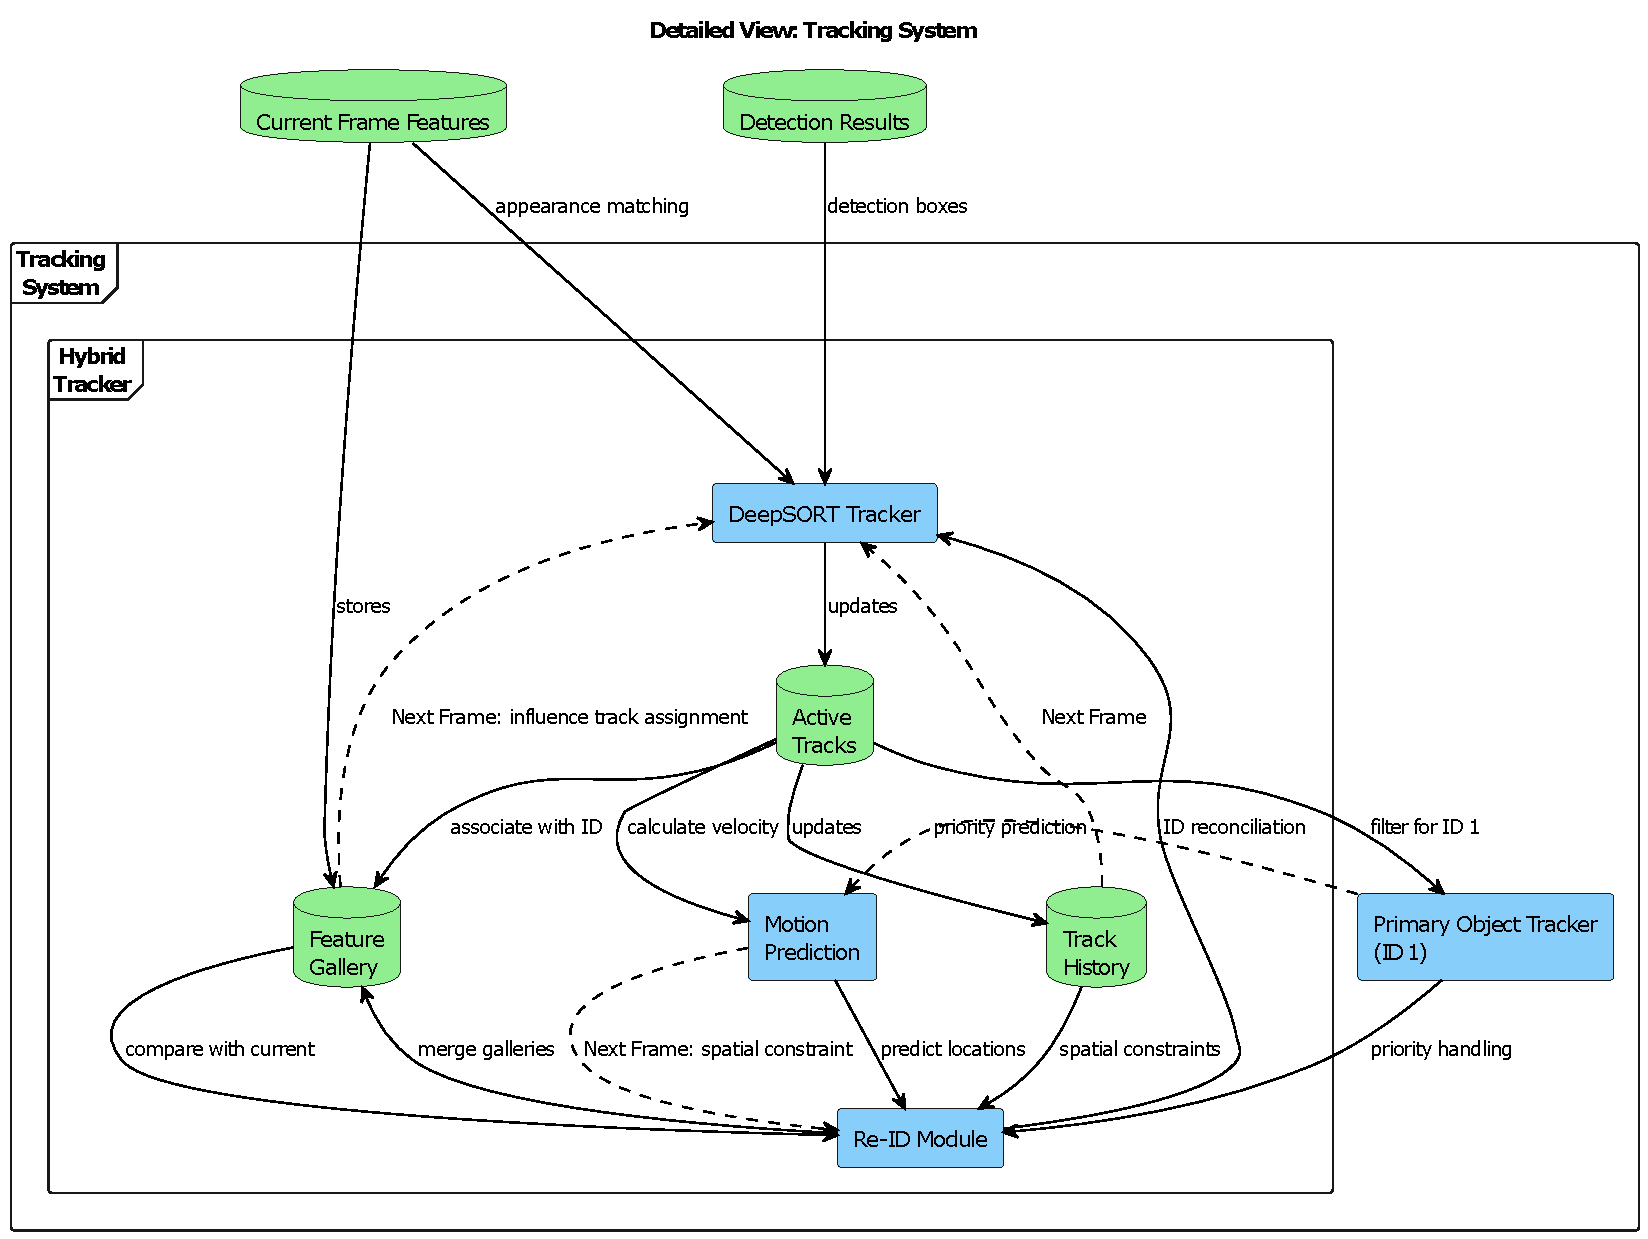
\includegraphics{diagrams/tracking_system_pipeline_diagram0-plantuml-svg-converted-to.pdf}}
\end{center}
\subsubsection{DINOv2 ViT-B/14}
Our primary feature extractor is the DINOv2 ViT-B/14 model, which generates a 768-dimensional feature vector. These features are L2-normalized to provide a compact and robust "visual fingerprint."
\subsubsection{ResNet50 Fallback}
In cases where DINOv2 may not be available or suitable, the system can fall back to a ResNet50 model, which produces 2048-dimensional feature vectors.

\subsection{Short-Term Tracking}
For frame-to-frame association, we employ the DeepSORT algorithm. DeepSORT is effective for handling short-term occlusions and smooth motion.
\subsubsection{Kalman Filtering}
DeepSORT uses Kalman filters to predict the motion of each object, estimating its state (position, velocity, etc.) in the current frame based on its state in the previous frame.
\subsubsection{Data Association (Hungarian Algorithm)}
Detections in the current frame are associated with existing tracks using a cost matrix that combines motion (predicted vs. detected position) and appearance similarity (from DeepSORT's internal Re-ID model). The Hungarian algorithm is used to find the optimal assignment that minimizes the total cost.

\subsection{Long-Term Re-identification}
To handle longer occlusions or when objects re-enter the scene after a significant absence, a more powerful Re-ID mechanism is employed, using the features extracted by DINOv2 or ResNet50.
\subsubsection{Feature Gallery}
A feature gallery is maintained for each tracked object. This gallery stores a deque of recent appearance features (embeddings) for that object.
\subsubsection{Online Re-identification}
When a new track is initiated by DeepSORT (i.e., a detection cannot be associated with an existing track), its features are compared against the galleries of recently inactive tracks. Cosine similarity is used to measure the distance between feature vectors. If a strong match is found below a certain threshold, the new track is assigned the ID of the inactive track.
\subsubsection{Offline Re-identification Refinement}
Periodically (e.g., every \texttt{re\_id\_interval} frames), a more comprehensive offline Re-ID process is performed. This involves comparing the feature galleries of all currently active tracks with those of all inactive tracks. If a strong similarity suggests that an active track and an inactive track actually represent the same object (a fragmented track), their IDs are merged. This helps consolidate identities over longer periods.

\subsection{Primary Object Tracking}
A key feature of the HLT-MOT system is its focus on robustly tracking a designated "primary object" (typically assigned ID 1).
\subsubsection{Initialization}
The first object detected in the scene is usually designated as the primary object.
\subsubsection{Dedicated Feature Management}
The system may employ specific strategies for managing the feature gallery of the primary object, potentially with more stringent update criteria or a larger gallery size.
\subsubsection{Enhanced Re-ID Criteria}
Stricter matching thresholds or additional consistency checks (like IoU) might be applied when attempting to re-identify the primary object to ensure high confidence.

\section{Core Components}
The HLT-MOT system is modular, with several key Python components orchestrating the tracking process.

\subsection{\\texttt{HybridTracker}}
This is the main class that encapsulates the overall tracking logic. It integrates the object detector, feature extractor, DeepSORT, and the custom long-term Re-ID mechanisms. It manages track states, ID assignments, feature galleries, and coordinates the online and offline Re-ID processes.

\subsection{\\texttt{FeatureExtractor}}
This module is responsible for loading the appearance feature extraction model (DINOv2 or ResNet50). It handles image preprocessing (cropping, resizing, normalization) and computes the L2-normalized feature embeddings for detected objects using PyTorch.

\subsection{\\texttt{YOLODetector}}
This component acts as a wrapper for the YOLO object detection models. It handles model loading (including TensorRT versions), pre-processing input frames, running inference, and post-processing detections (e.g., Non-Maximum Suppression).

\subsection{DeepSORT Integration}
The system utilizes the \texttt{deep\_sort\_realtime} library for its short-term tracking capabilities. The `HybridTracker` class interfaces with DeepSORT, providing it with detections and receiving track updates.

\section{Optimization Techniques}
To achieve real-time or near real-time performance, several optimization strategies are employed.

\subsection{Batch Processing}
When multiple objects are detected in a frame, feature extraction is performed in a batch operation where possible, leveraging the parallel processing capabilities of GPUs.

\subsection{GPU Acceleration}
CUDA is utilized for computationally intensive tasks:
\begin{itemize}
    \item Object detection inference (YOLO with PyTorch/TensorRT).
    \item Feature extraction (DINOv2/ResNet50 with PyTorch).
    \item Batch cosine distance calculations for feature matching during Re-ID.
\end{itemize}

\subsection{Numba Optimization}
For certain CPU-bound calculations that can benefit from Just-In-Time (JIT) compilation, Numba is used. This includes:
\begin{itemize}
    \item Intersection over Union (IoU) calculations.
    \item Spatial distance calculations.
\end{itemize}

\subsection{Selective Feature Extraction and Updates}
To reduce computational load, especially when tracking a primary object, feature extraction might be performed more selectively. For instance, features for non-primary objects might be extracted less frequently or only when Re-ID is critical. Motion predictions and gallery updates can also be prioritized for the primary object.

\section{Spatial-Temporal Consistency}
Beyond appearance similarity, spatial and temporal cues are vital for robust tracking and Re-ID.

\subsection{Intersection over Union (IoU) Checking}
IoU is used to measure the overlap between bounding boxes. It serves as a spatial consistency check during data association and Re-ID, helping to disambiguate tracks that are spatially close or to verify if a re-identified object's position is plausible.

\subsection{Motion Prediction and Track History}
The Kalman filter in DeepSORT provides short-term motion prediction. The `HybridTracker` also maintains a history of recent positions for each track. This history can be used for:
\begin{itemize}
    \item Simple motion extrapolation to predict an object's likely position if it's temporarily lost.
    \item Spatial constraints during Re-ID (e.g., a re-appearing object should be reasonably close to its last known position).
\end{itemize}

\section{Experimental Setup}
% This section should be filled in by the author.
% Describe the datasets used for evaluation (e.g., MOTChallenge, custom videos).
% Specify the evaluation metrics (e.g., MOTA, MOTP, IDF1, HOTA).
% Detail the hardware and software environment.
% Mention parameter settings for the tracker.

\section{Results and Discussion}
% This section should be filled in by the author.
% Present quantitative results on the chosen datasets and metrics.
% Provide qualitative results (e.g., example tracking sequences, failure cases).
% Discuss the performance of the system, highlighting strengths and weaknesses.
% Analyze the impact of different components (e.g., DINOv2 vs. ResNet50, effect of offline Re-ID).

\section{Conclusion and Future Work}
This paper presented the HLT-MOT system, a hybrid approach to long-term multi-object tracking. By combining DeepSORT for short-term association with a DINOv2-based feature extractor for robust long-term Re-ID, and incorporating optimizations and a focus on primary object tracking, the system aims to provide consistent identities over extended periods.

Future work could explore:
\\begin{itemize}
    \\item Fine-tuning Re-ID models on domain-specific data.
    \\item Implementing more sophisticated motion models.
    \\item Exploring graph-based global optimization for track association.
    \\item Extending to multi-camera tracking scenarios.
\\end{itemize}

\bibliographystyle{IEEEtran}
\bibliography{references}

% ...existing code...
\end{document}
